%%%%%%%%%%%%%%%%%%%%%%%%%%%%%%%%%%%%%%%%%%%%%%%%%%%%%%%%%%%%%%%%%%%%%%%
% Based on IEEE the conference template available                     %
% at https://www.ieee.org/conferences/publishing/templates.html       %
% Adapted for the Data Science Lab course at Politecnico di Torino    %
% by Giuseppe Attanasio, Flavio Giobergia                             %
% 2020, DataBase and Data Mining Group                                %
%%%%%%%%%%%%%%%%%%%%%%%%%%%%%%%%%%%%%%%%%%%%%%%%%%%%%%%%%%%%%%%%%%%%%%%

\documentclass[conference]{IEEEtran}
\usepackage{cite}
\usepackage{amsmath,amssymb,amsfonts}
\usepackage{algorithm}
\usepackage{algorithmic}
\usepackage{graphicx}
\usepackage{textcomp}
\usepackage{xcolor}
\usepackage{subfigure}

\begin{document}

\title{
Lab G7: Natural selection
}

\author{
    \IEEEauthorblockN{Emanuele Pietropaolo}
    \IEEEauthorblockA{
        \textit{Politecnico di Torino} \\
        Student id: s319501 \\
        emanuele.pietropaolo@studenti.polito.it
        }
}

\maketitle
% \begin{abstract}
    
    
% \end{abstract}

\section{Problem overview}

    In nature, a population starts to evolve because of environmental factors. 
    %
    These factors affect the chances of an individual surviving. 
    %
    There can be many different variables that affect this chance, such as scarcity of resources, predators, disease, etc. 
    %
    Some individuals can develop resistance to one or more of these factors, improving their ability to survive and reproduce, and pass this resistance on to new generations. 

    One of the key elements of natural selection is survival against predators. Many species develop a symbiotic relationship known as `\textit{prey-predator}`. 
    %
    There are predators that evolve for the purpose of being more effective at preying on a particular species, and that species, the prey, is then selected to evolve caratteristic that will allow it to better survive the predator attacks.

    This report analyses how natural selection can affect this relationship between two species, and in particular which parameters have more influence on life expectancy and the actual lifespan of individuals. 

    %1. Introduci una capacità di carico: In natura, l'ambiente ha una capacità di carico massima, che è il numero massimo di individui che l'ambiente può sostenere. Quando la popolazione raggiunge la capacità di carico, la crescita della popolazione rallenta o si ferma. Potresti introdurre un concetto simile nella tua simulazione. Ad esempio, potresti fare in modo che il tasso di riproduzione diminuisca quando la popolazione è vicina alla capacità di carico.

    % 2. Variazione del tasso di riproduzione: Attualmente, tutti gli individui nella tua simulazione hanno lo stesso tasso di riproduzione. In natura, tuttavia, il tasso di riproduzione può variare tra gli individui. Potresti introdurre una certa variazione nel tasso di riproduzione nella tua simulazione. Ad esempio, potresti fare in modo che il tasso di riproduzione di un individuo sia una funzione del suo "lifetime".

    % 3. Mortalità dipendente dalla densità: In natura, la mortalità spesso aumenta con la densità della popolazione. Potresti introdurre un concetto simile nella tua simulazione. Ad esempio, potresti fare in modo che la probabilità che un individuo muoia aumenti quando la popolazione è grande.

    % 4. Riproduzione sessuale: Attualmente, sembra che stai simulando una riproduzione asessuata, in cui ogni individuo produce un figlio da solo. Potresti considerare di simulare la riproduzione sessuale, in cui due individui producono un figlio insieme. Questo potrebbe introdurre ulteriori dinamiche interessanti nella tua simulazione.

\section{Proposed approach}

\subsection{Assumptions}

    Simulating such a complex process can be a challenging task. For this reason, some assumptions have been made:

    % \begin{figure}[!b]
    %     \centering
    %     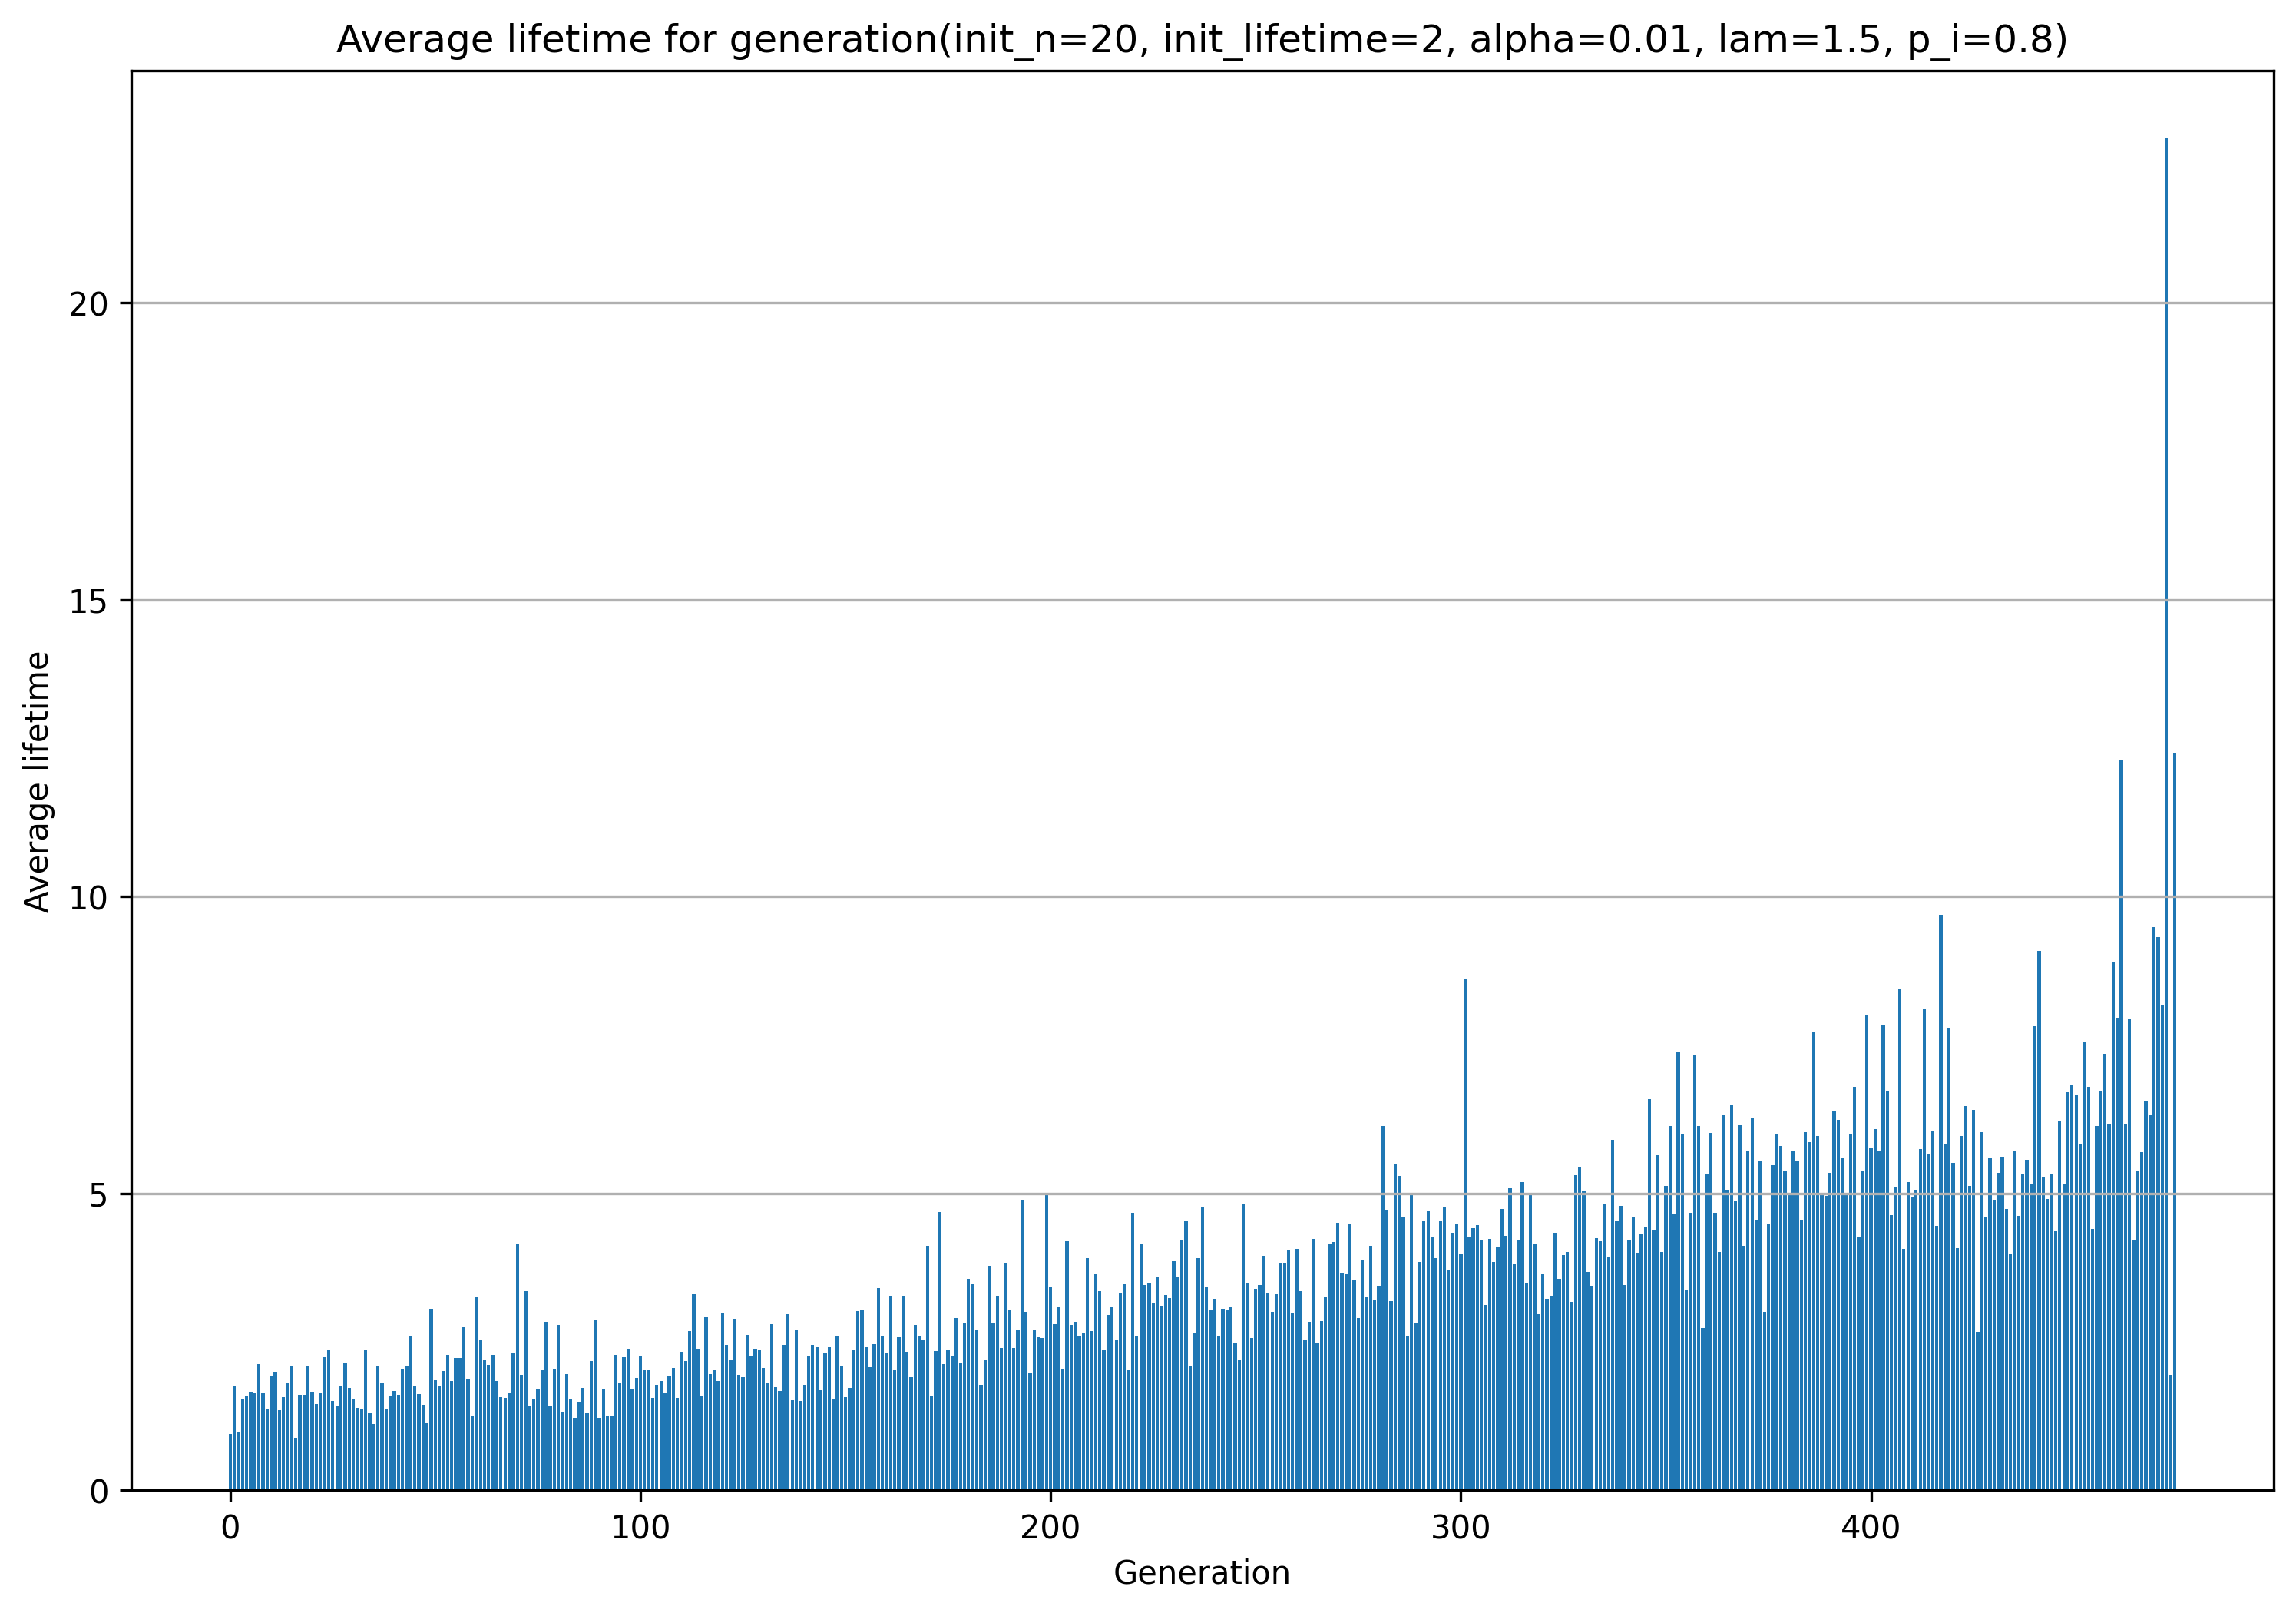
\includegraphics[width=\columnwidth]{media/in_p_20_in_lt_2_a_0.01_l_0.5_p_i_0.2/lf.png}
    %     \caption[short]{Lifetime evolution with low $p_i$ and low $\lambda$}
    %     \label{fig:lf_low}
    % \end{figure}

    \begin{itemize}
        \item \textbf{Reproduction:} in nature there are many different forms of reproduction. Most require two individuals of the same species.
        %
        In this study, the species considered are mammals, so the type of reproduction modelled is \textit{sexual reproduction}.  
        %
        In order to have a \textit{birth event}, a female must mate with a male of the same species, and a mating event can only occur if the two individuals are in the same place at the time when the female is in heat. 
        \item \textbf{Reproduction rate ($\lambda$):} The reproductive rate is considered to be the rate at which a female will have periods of being in heat ($\lambda$). The time between heat periods was generated by an exponential distribution, assuming that the total heat process of a female follows a Poisson distribution.
        \item \textbf{Puberty time:} each individual cannot participate in mating events until they reach puberty. This element adds a level of realism and prevents the population from becoming incrontrollably overgrown.
        \item \textbf{Number of new born:} each female can give birth to more than one individual per birth event. Each individual has its own life expectancy variable and the number of newborns is generated from a Poisson distribution, knowing the average number of children for each species.
        \item \textbf{Pregnancy:} for a new birth event to occur, a period of time is considered between the mating event and the actual birth event. This period represents the gestation period. The actual birth event will only occur if the female survives to the scheduled birth event. 
        \item \textbf{Sterility probability:} at birth time, is generated a probability that the newborn will be sterile. This will act as upper bound for the number of individuals for a given species in a realistic way. This probability depends on the number of individual in the moment of the birth event and on an input parameters.
        \item \textbf{Improvement over generation:} this is the process that models how resistance has been passed on to new generations. Each newborn receives a life expectancy from its parents, which is used to generate its lifetime variable. The life expectancy of the new born is the average life expectancy of the two parents. There is a possibility that this life expectancy will be greater than the average life expectancy of the parents ($p_i$). In this case, it is randomly generated from a uniform distribution between the average life expectancy of the parents and the average life expectancy of the parentst multiplied by a factor ($1+\alpha$). Otherwise it is generated from a uniform distribution between 0 and the average life expectancy of the parents.
    \end{itemize}

\subsection{Models}

    The simulation takes into account various factors to create a realistic scenario and there are three main models that have been developed:

    \begin{itemize}
        \item \textbf{Fight model:} fight events represent the hunting of predators. The hunt is modelled as a group hunt: each time a predator wants to hunt a prey, it first searches for other individuals of its species. A winning probability is generated and given to each individual taking part in the hunt, so the more predators are in the group, the more chances they have to win the fight. The maximum number of predators in a group is 3. Not all predators are interested in taking part in the fight, some of them may have eaten recently. The winning probability generated before each fight depends on the ratio between the number of predators and prey in the entire population. This represents the hunting pressure that the predators exert on the prey population: the lower the pressure, the higher the chance of finding prey that are not ready to fight, and therefore the higher the probability of winning. The higher the pressure, the higher the change that the prey will be alert and the predator will compete higher, so the lower the probability of winning. At every hunt, the predator will chose the youngest individual to fight.
        \item \textbf{Survival model prey:} as discussed above, the prey will survive based on the winning probability given to each predator for the fight model, but another consideration is also taken into account: there is a probability that a prey can hide from the predators before the fight even happens. In fact, when the predators are looking for prey, only those prey that are not hiding are available for the fight. The probability of hiding depends again on the ratio of predators to prey, this will act as a response of the prey in case of high hunting pressure exerted by the predators. This almost always prevents the complete extinction of the prey population, as the probability is very high when the number of prey is low. 
        \item \textbf{Survival model predator:} Survival model: The predator must eat often or it will starve. Starvation events are generated to keep a predator alive for a while to allow it to hunt, if the predator doesn't eat in that time the starvation event will cause a death event. There is a common problem in predator-prey simulations that causes the predator population to go extinct when the prey population reaches a minimum. To prevent this from happening too often, the death event is triggered with a certain probability, which again depends on the ratio between the number of predators and prey in the whole population. This will represent the possibility that a predator has eaten something else in response to the scarcity of prey. In the majority of cases, this will prevent the premature termination of the predator population.
        \item \textbf{Mobility model:} the main idea behind the mobility model is that each individual moves randomly around the world. The rate of movement is an input parameter. The world is modelled as a graph where each node corresponds to a land area. Each time a movement event occurs for an individual, it randomly chooses a neighbouring node and changes it's current location variable. The graph is modelled as a dictionary and it also stores all the living individuals in their positions. The mobility model will affect the mating events, in fact, every time a female in heat randomly changes location she starts looking for a male to reproduce with and every time a male randomly changes location he starts looking for a female in heat. The mobility model also affects the fighting model, because when a predator starts to hunt, it can engage with other individuals present in its land area. 
    \end{itemize}

\subsection{Events}

    \begin{itemize}
        \item \textbf{Birth:} the birth event will add a newborn to the population and to the world. It takes as parameters the current\_time, the newborn reference, the move\_rate, the input limit population to calculate the sterile probability, and also the FES, the population and the world reference to update their states. At birth the firsts move event and in\_heat event are scheduled and if the newborn is a predator also the first fight and starve event. 
        \item \textbf{Death:} the death event will remove an individual from the population and from the world.
        \item \textbf{Start in heat:} the start in heat event will occur only for female and put the female in a reproductive state. In this event is first checked if the female is still alive, and if so it starts to look for male in the same position to have a mate event. Also a stop in heat event is scheduled.
        \item \textbf{Stop in heat:} this event will end the reproductive state for a female if she didn't have a mate event in the meantime. The next start in heat event is scheduled.
        \item \textbf{Move:} this event will cause a random move in the world for a specific individual. The move event will trigger mate events as described above
        \item \textbf{Mate:} in this event a male look for a female that is in a reproductive state. If the mating has been successful, it generate a number of newborns as described above, a birth is scheduled and the female is put on pregnancy (this will mean that she can't have in-heat period in the mean time)
        \item \textbf{Fight:} as described above, this event trigger the fight model
        \item \textbf{Starve:} as described above.
    \end{itemize}

\subsection{Scenario and input parameters}

    In this simulation two species as been taken into consideration. A long study as been taken in order to let them find the right condition to have a equilibrium state. For this reason a scenario where there are no natural selection is also shown in the results as baseline.
    
    \begin{figure}[!ht]
    \centering
    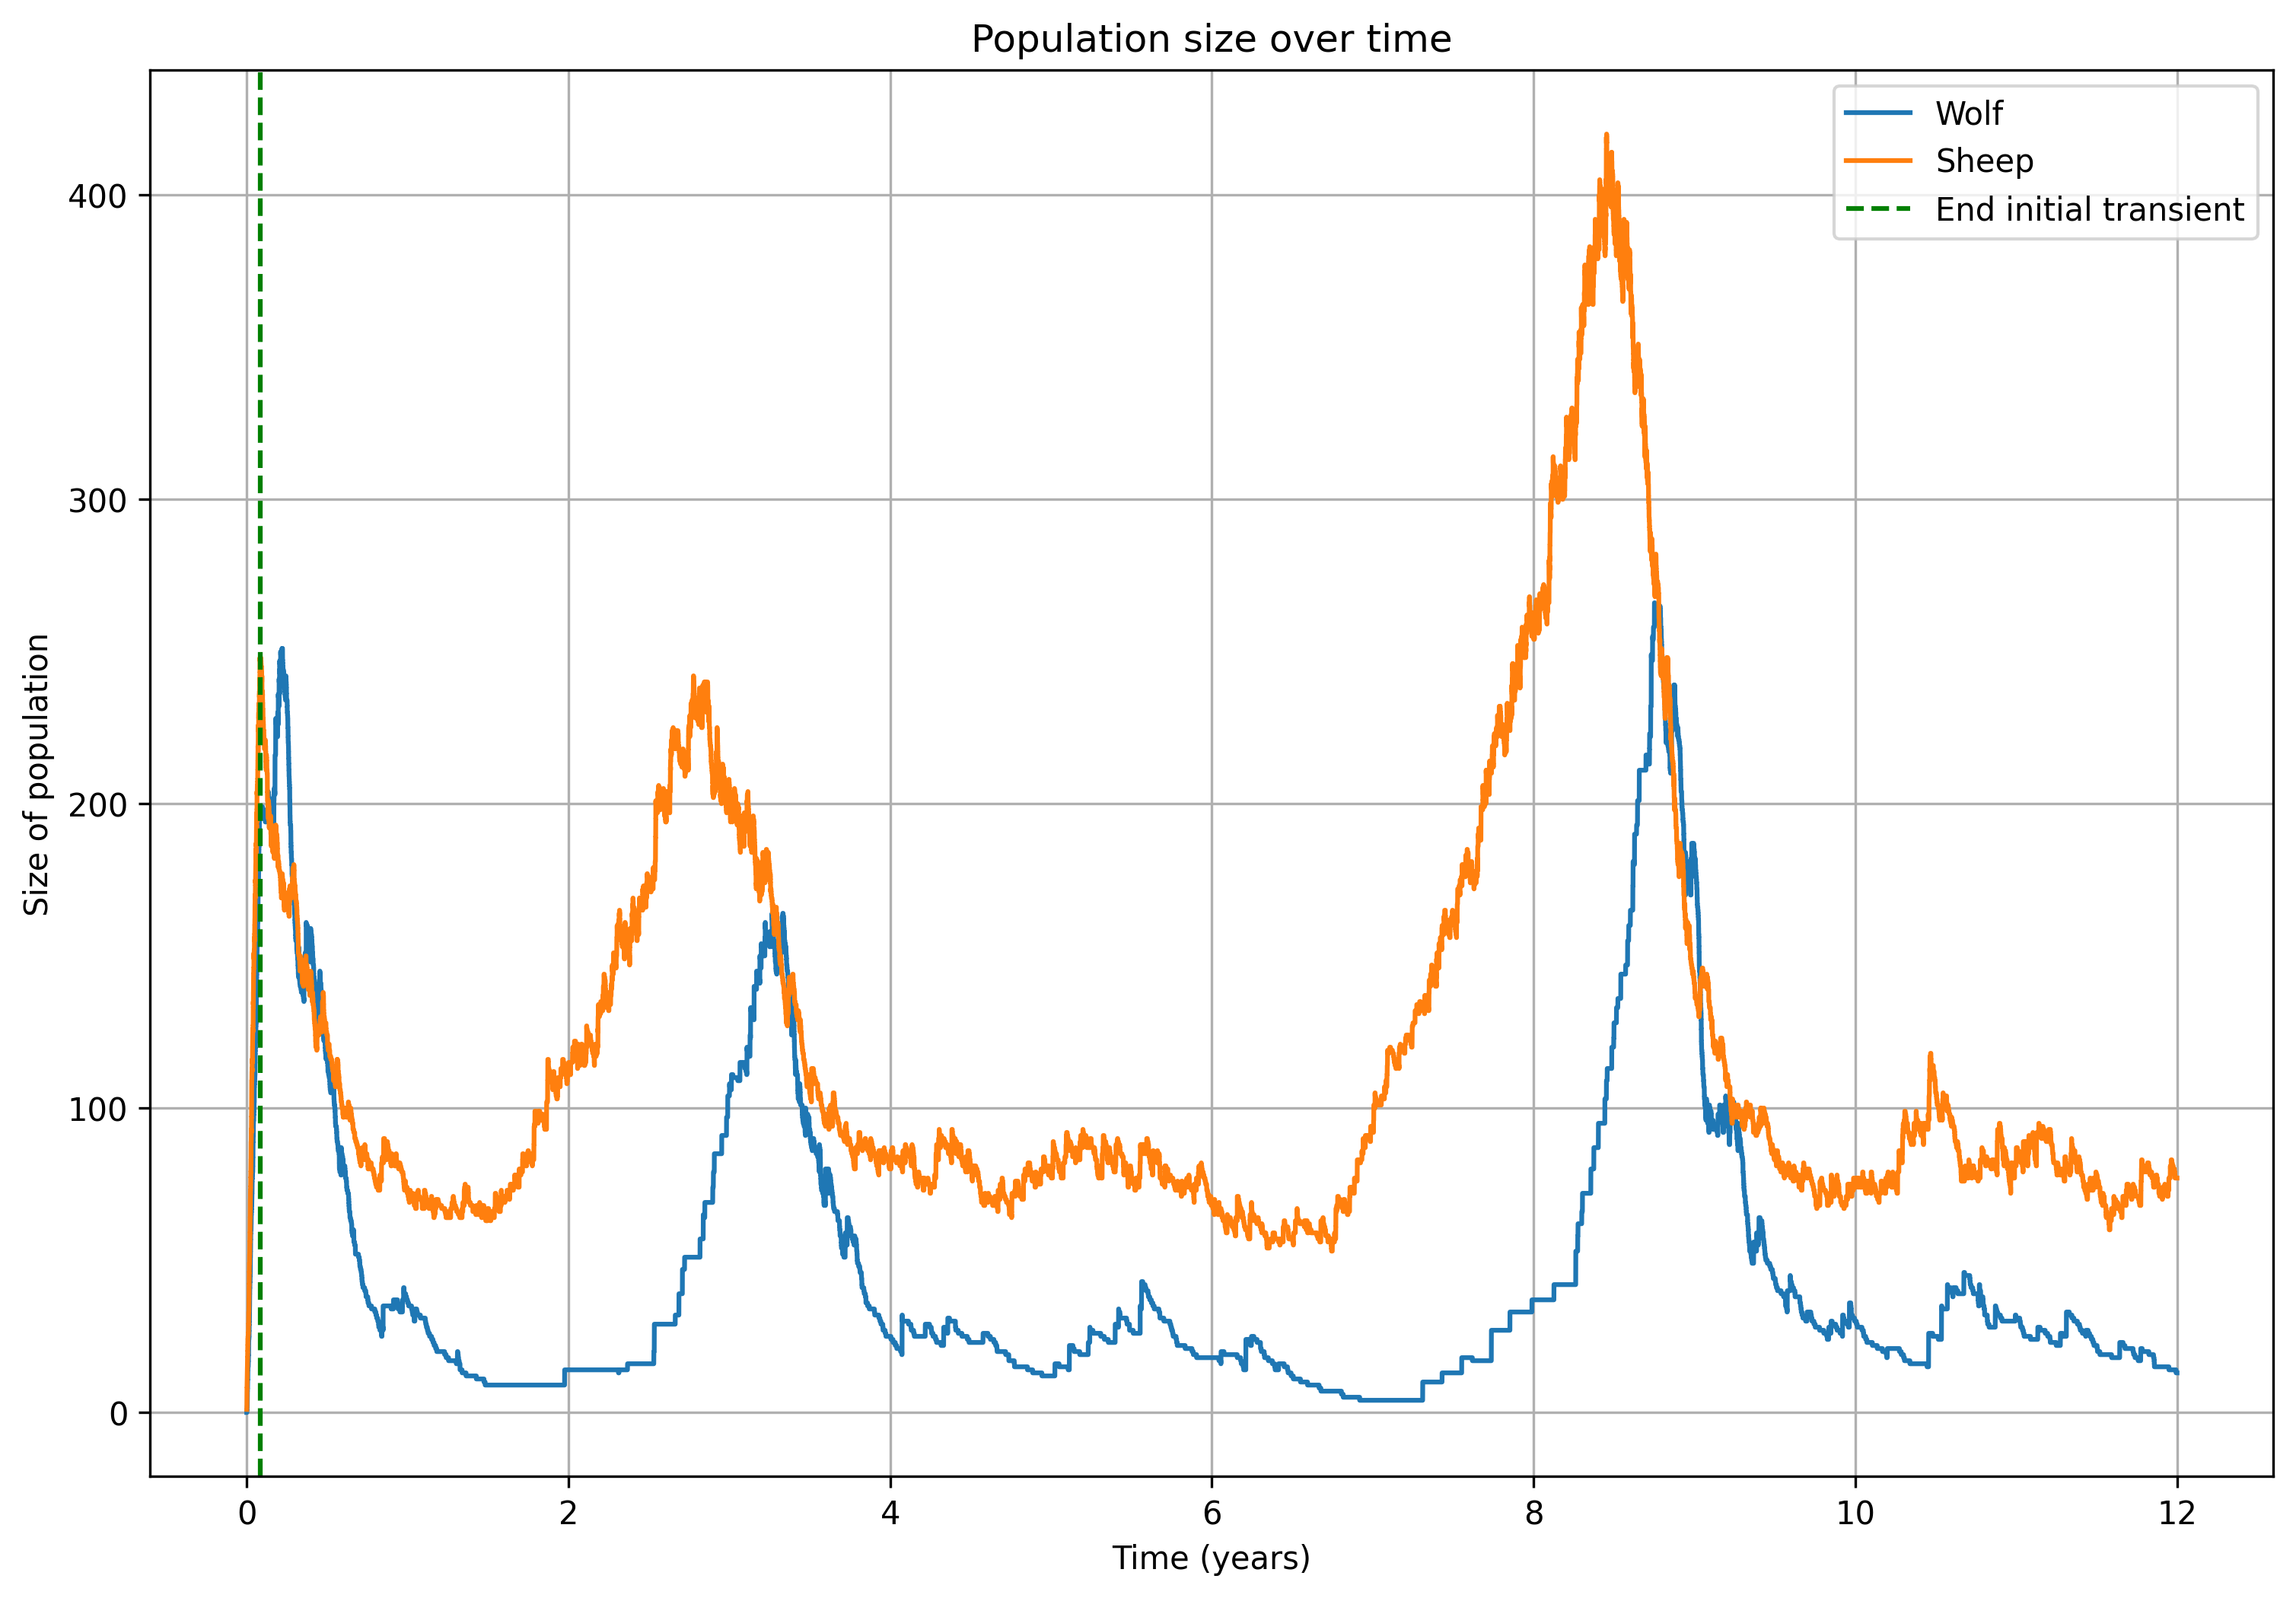
\includegraphics[width=\columnwidth]{media/0_11-02-2024_19-13-55-022905_pop_time_species}
    \caption[short]{Simulation without natural selection}
    \label{fig:no_sel}
    \end{figure}

    The predator species is a fox, with a initial life expectancy of 5 years, a reproduction rate of 4 times a year and an average number of newborns of 6 individuals. Its puberty will last the 15\% of the life expectancy, it can remain at least 21 days without food and goes hunt every 7 days on average. The starvation rate is set to every 31 days on average but not less than 21. The day between hunts is set to be 3 days and the pregnancy last for 40 days.

    The prey species is a rabbit, with an initial life expectancy of 4 years, a reproduction rate of 5 times a year and an average number of newborns of 3 individuals. It puberty las the 15\% of the life expectancy ad its pregnancy last for 25 days. 

    For both species the in heat period last for 7 days.

\section{Results}

    \subsection{Simulation without natural selection}

    As can be seen in Fig.\ref{fig:no_sel} the simulation is able to reach the stable equilibrium of its population. It can be seen how as the prey population grow follows a growth in the predator population and when it decrease after a while it decrease also the predator population.

    \subsection{Life expectancy predator}

    \begin{figure}[!ht]
    \centering
    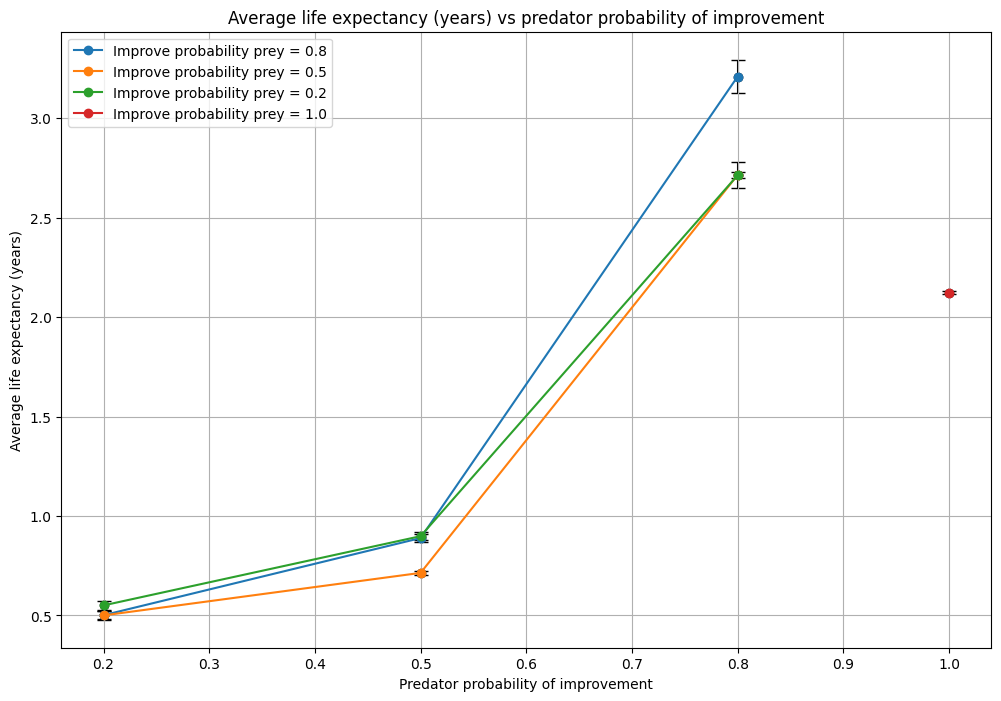
\includegraphics[width=\columnwidth]{media/lf_predator.png}
    \caption[short]{Life expectancy predator}
    \label{fig:lf_predator}
    \end{figure}

    It can be seen in Fig.\ref{fig:lf_predator} there is a trend that shown how the life expectancy of the predator rely on the probability of improvement. The interesting fact is that  it rely also in the life expectancy of the prey. 

    % \begin{figure}[!ht]
    % \centering
    % 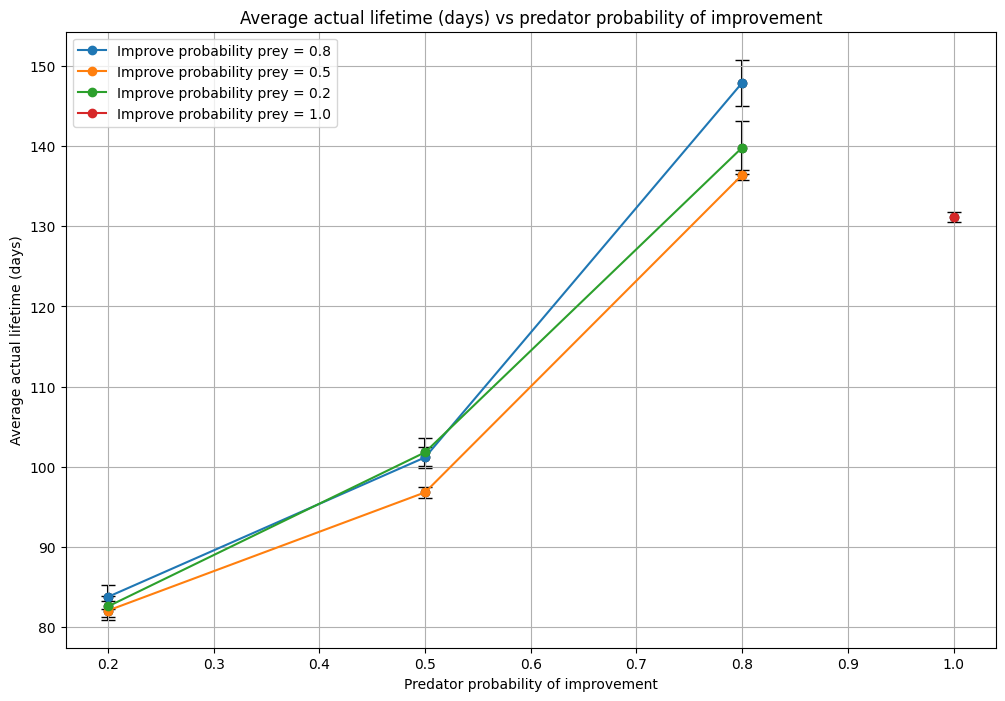
\includegraphics[width=\columnwidth]{media/l_predator.png}
    % \caption[short]{Actual lifetime predator}
    % \label{fig:l_predator}
    % \end{figure}

    \begin{figure}[!ht]
    \centering
    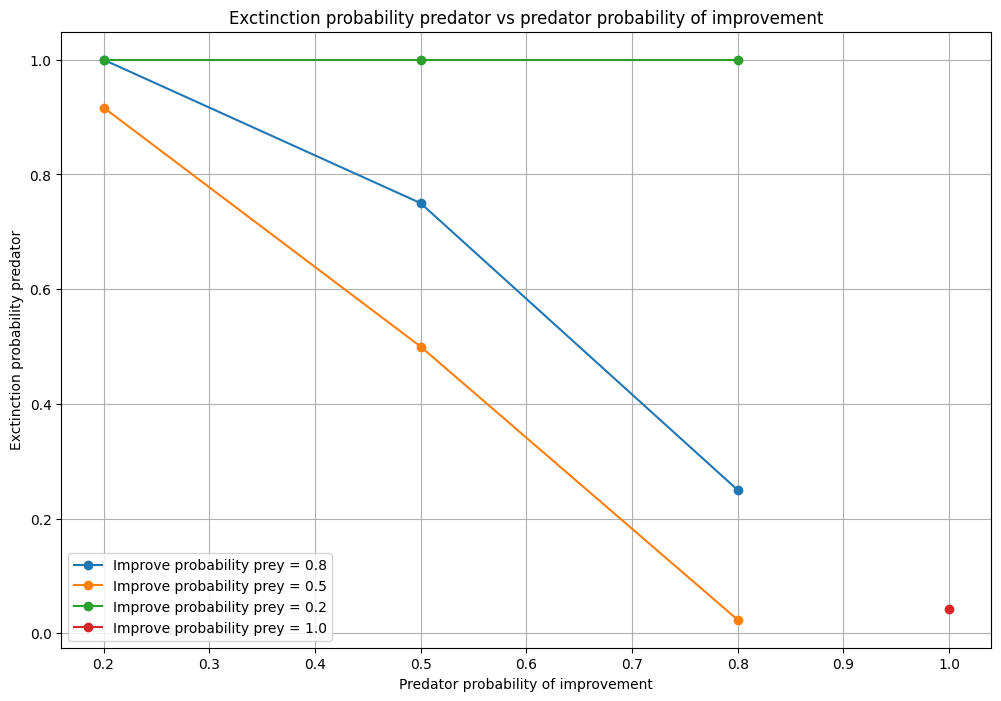
\includegraphics[width=\columnwidth]{media/exctinct_prob_predator.png}
    \caption[short]{Exctinction probability predator}
    \label{fig:ex_predator}
    \end{figure}

    \subsection{All studied cases}

    \begin{figure}[!ht]
    \centering
    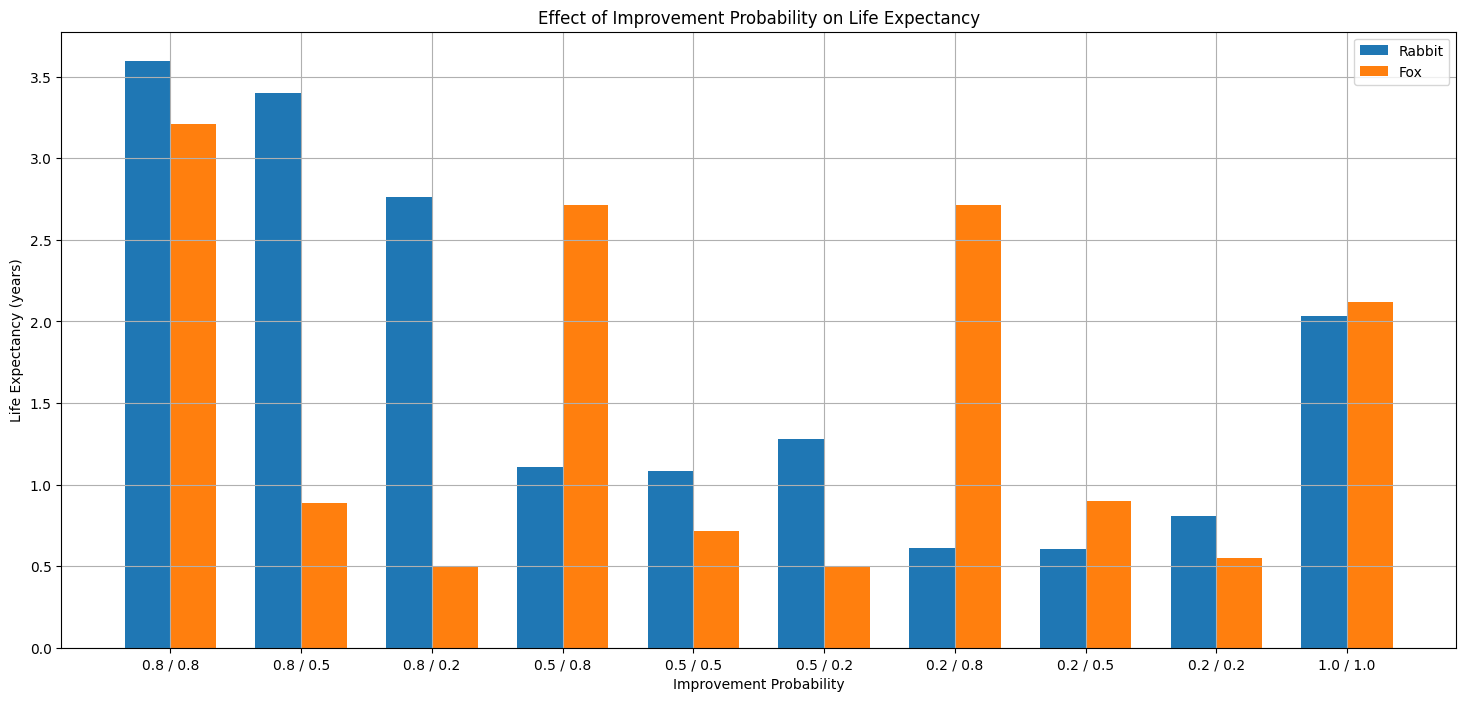
\includegraphics[width=\columnwidth]{media/overal_lf.png}
    \caption[short]{Life expectancy for all the cases}
    \label{fig:lf_all}
    \end{figure}

    \begin{figure}[!ht]
    \centering
    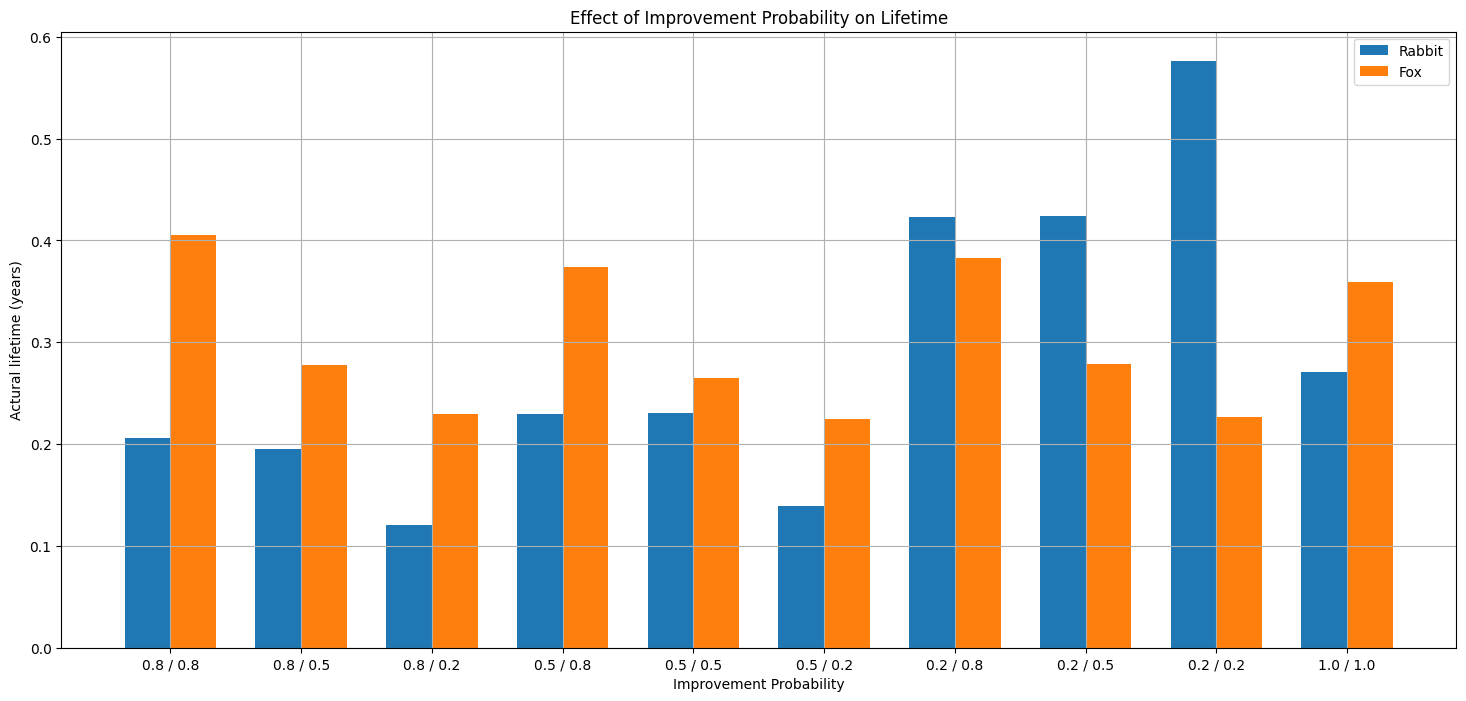
\includegraphics[width=\columnwidth]{media/overal_l.png}
    \caption[short]{Actual lifetime for all the cases}
    \label{fig:l_all}
    \end{figure}

    The case where the improvement probability is set to both 1 serve as the simulation without natural selection.

%\bibliography{bibliography}
%\bibliographystyle{ieeetr}

\end{document}
